
\begin{frame}[fragile]

 \heading{Calculate an ensemble of pendulums}

 \begin{lstlisting}[basicstyle=\scriptsize\ttfamily]
typedef mtl::dense_vector<double> vector_type;
typedef mtl::multi_vector<vector_type> state_type;
typedef runge_kutta4<state_type,double,state_type,double,
  vector_space_algebra,default_operations> stepper_type;

state_type X(N, 2);
vector_type Eps(N), Omega(N);

// initialize x, Eps, Omega
integrate_const(stepper(), ensemble(Eps, Omega, 0.1) ,
    X, 0.0, t_max, dt);
 \end{lstlisting}

\vspace{2ex}

\centerline{Memory layout:}

\vspace{1ex}

\centerline{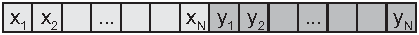
\includegraphics[draft=false,width=0.7\textwidth]{memory_layout2.pdf}}

\vspace{2ex}

\centerline{Everything seems easy!}
\vspace{2ex}
\centerline{{\bf But} how does {\tt ensemble} look like?}
 

\end{frame}




\begin{frame}[fragile]

 \heading{Ensemble of nonlinear pendulums}

 \begin{lstlisting}[basicstyle=\scriptsize\ttfamily]
struct ensemble
{
  const vector_type &m_eps, &m_omega;
  double m_mu;

  ensemble(const vector_type &eps,const vector_type &omega,
    double mu)
      : m_eps(eps), m_omega(omega), m_mu(mu) { }

  void operator()(const state_type &x, state_type &dxdt,
    double t)
  {
    dxdt.at(0)= x.at(1);
    dxdt.at(1)= -sin(x.at(0)) - m_mu*x.at(1) + m_eps*sin(m_omega*t);
  }
};
 \end{lstlisting}

\end{frame}

\begin{frame}
  \heading{What is MTL4?}
  \begin{itemize}
  \item Matrix Template Library v4
  \item A Library for linear algebra
  \item It provides an intuitive interface
  \item Similar to Matlab
    \begin{itemize}
    \item Translators Matlab $\rightarrow$ MTL4 in progress
    \end{itemize}
  \item Simplicity without sacrificing performance
  \item Portability with little or no code change

  \end{itemize}

\end{frame}


\subsection{Our Vision of Portable Programming}

\swvision{Folie1}
\swvision{Folie2}
\swvision{Folie3}
\swvision{Folie4}
\swvision{Folie5}
\swvision{Folie6}
\swvision{Folie7}
\swvision{Folie8}
\swvision{Folie9}
\swvision{Folie10}
\swvision{Folie11}
\addtocounter{framenumber}{1}




\begin{frame}
  \heading{Challenges with CUDA}
  \begin{itemize}
  \item No support for complex,
  \item No mixed arithmetic,
  \item Intrinsically only flat copies,
    \begin{itemize}
    \item Limits applicability of user types,
    \end{itemize}
  \item Many algorithms difficult or impossible on GPU

  \end{itemize}

\end{frame}



\begin{frame}
  \heading{Portability}
  \begin{itemize}
  \item Same abstractions and interfaces for
    \begin{itemize}
    \item Sequential MTL4,
    \item CUDA-MTL4, and
    \item Parallel MTL4.
    \end{itemize}
  \item Entirely generic design
    \begin{itemize}
    \item In fact, most of the code is identic
    \end{itemize}


  \end{itemize}

\end{frame}

\begin{frame}
  
\end{frame}